\section{Описание раздела <<Товары>>}\label{sec:sec14_1}
\begin{enumerate}[\thesection .1]
\item Модуль служит для просмотра информации об остатках товара на центральных складах предприятия (рис.\ref {pic:pic15_1}). Также поддерживаются следующие функции: 
\begin{itemize}
	\item Просмотр списка товаров (с возможностью просмотра остатков товаров на вэн-складе \footnote{Вэн-склад - мобильный склад торгового представителя (кузов).} и на центральном складе);
	\item Просмотр детальной информации по товару;
	\item Установка единиц измерения товаров;
	\item Просмотр цен товаров (прайс-листов);
\end{itemize}
\item В каждом элементе списка содержатся:
\begin{itemize}
	\item Краткое наименование товара;
	\item Остаток товара на вэн-складе;
	\item Остаток товара на центральном складе;
	\item Наименование единицы измерения.
\end{itemize}

\begin{figure}[!h]
	\begin{floatrow}
		\ffigbox{\caption{Окно Товары}\label{pic:pic15_1}}%
		{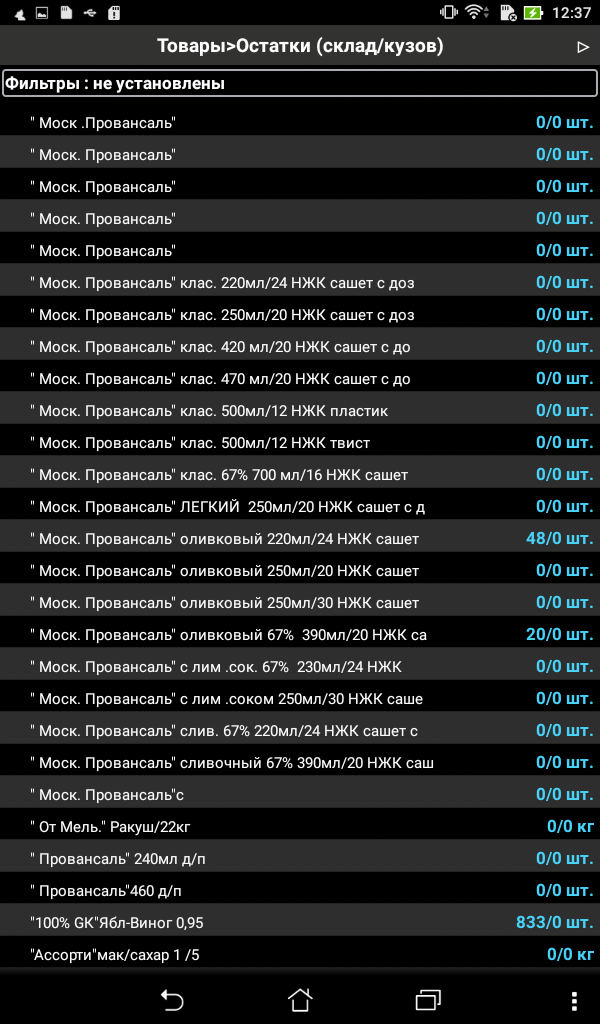
\includegraphics[width=0.8\linewidth]{scr15_1.png}}
		\ffigbox{\caption{Цены}\label{pic:pic15_2}}%
		{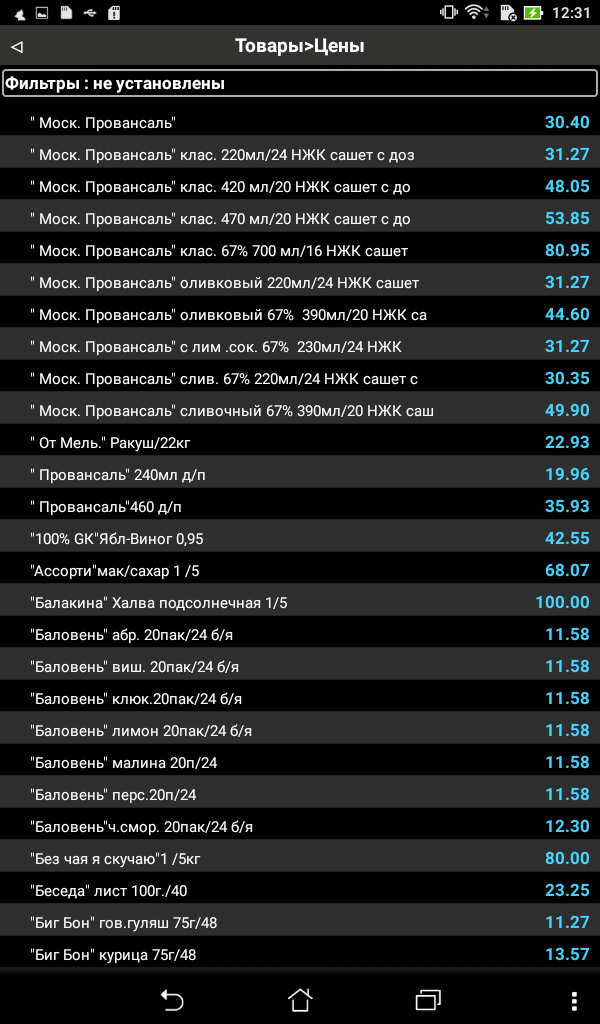
\includegraphics[width=0.8\linewidth]{scr15_2.png}}         
	\end{floatrow}
\end{figure}
\item Фильтры, доступные в окне: \footnote{Чтобы осуществить переход в окно выбора фильтров нужно произвести длительное касание в области фильтров. При коротком касании в области фильтров производится переход к окну выбора узла в иерархическом списке (фильтр «Каталог»).}
\begin{itemize}
	\item Каталог (фильтр по узлу номенклатурой иерархии);
	\item Количество (>0 или любое);
	\item Склад;
	\item MML;
	\item Атрибут;
	\item Значение;	
\end{itemize}
\item При скользящем касании справа - налево открывается окно просмотра цен (рис.\ref {pic:pic15_2}). 
В каждом элементе списка представлен товар и цена на него по прайс-листу, установленному в области фильтров.
Фильтры, доступные в окне просмотра цен товаров:
\begin{itemize}
	\item Каталог (фильтр по узлу номенклатурой иерархии);
	\item Прайс-лист (обязательный изменяемый фильтр);
	\item Склад;
	\item MML;
	\item Атрибут;
	\item Значение;	
\end{itemize}
\item Окно детальной информации о товаре
Для того чтобы перейти в окно просмотра детальной информации о товаре
\textbf{(Товары > Подробно)}  выберите товар кратким касанием в окне просмотра остатков товаров \textbf{(Товары > Остатки)}. При выборе товара в окне просмотра цен товаров \textbf{(Товары > Цены)} также происходит переход в окно \textbf{(Товары > Подробно)}
(рис.\ref {pic:pic15_3}).
\begin{figure}[!h]
	\begin{floatrow}
		\ffigbox{\caption{Окно просмотра детальной информации по товару}\label{pic:pic15_3}}%
		{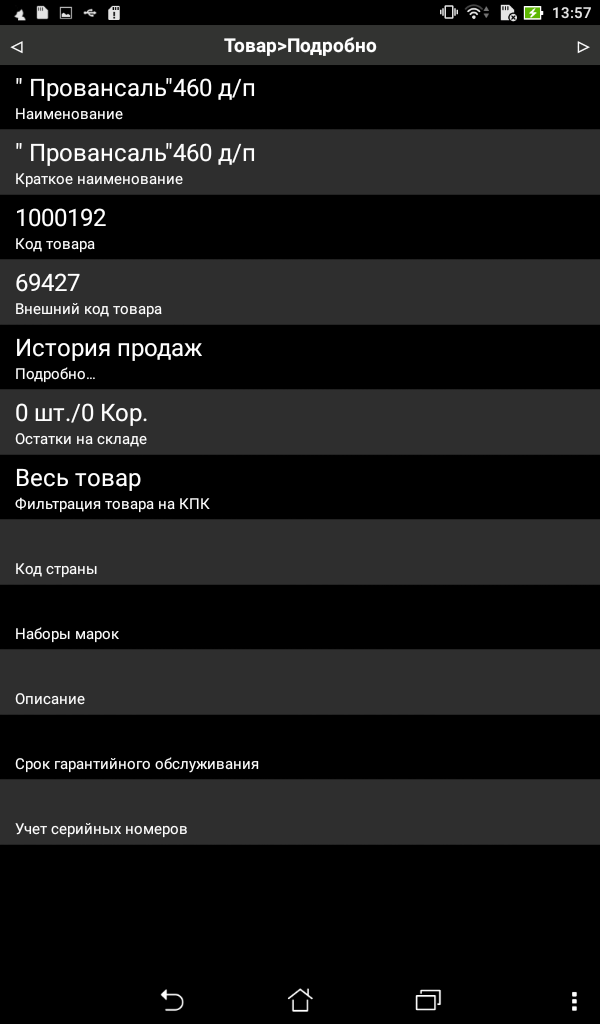
\includegraphics[width=0.8\linewidth]{scr15_3.png}}
		\ffigbox{\caption{Окно просмотра единиц измерения
				}\label{pic:pic15_4}}%
		{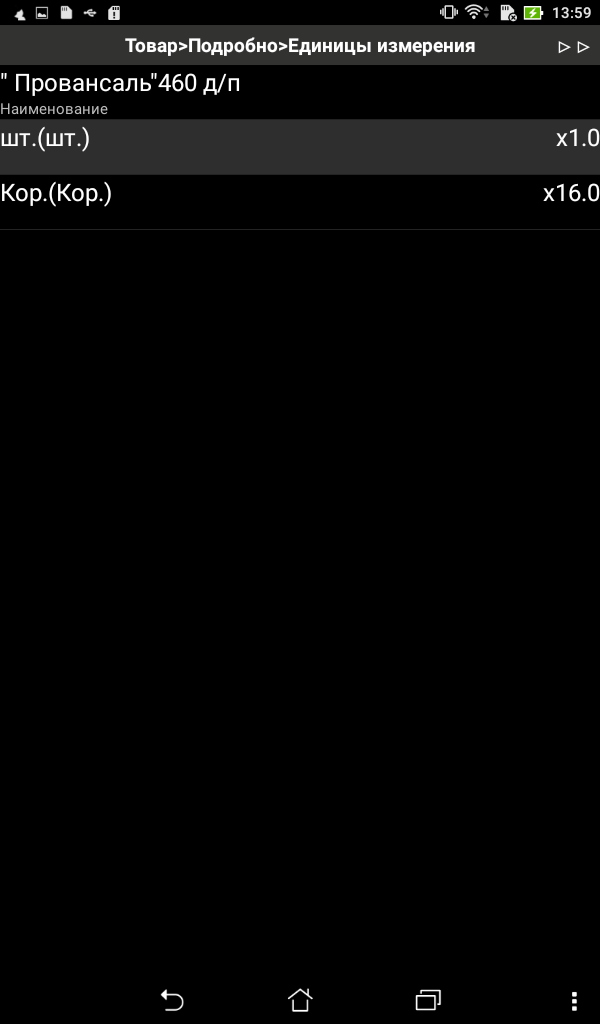
\includegraphics[width=0.8\linewidth]{scr15_4.png}}         
	\end{floatrow}
\end{figure}
В окне \textbf{(Товары > Подробно)} отображаются: 
\begin{itemize}
	\item Полное и краткое наименование товара;
	\item Код товара;
	\item Остатки на складе;
	\item Дополнительные атрибуты товара, сконфигурированные в конкретной системе.
\end{itemize}
\item При скользящем касании экрана слева - направо происходит переход в окно просмотра единиц измерения товара.(рис.\ref {pic:pic15_4}). 
В окне просмотра единиц измерения отображаются: 
\begin{itemize}
	\item Полное наименование товара;
	\item Cписок единиц измерений, присвоенных этому товару.
\end{itemize}
В каждом элементе списка содержится следующая информация:
\begin{itemize}
	\item Полное и краткое название ЕИ;
	\item Кратность ЕИ;
\end{itemize}
\end{enumerate}